\begin{figure}[ht]
    \centering
    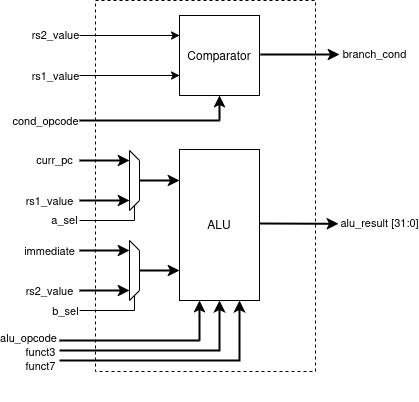
\includegraphics[scale=0.4]{IE_BD.png}
    \caption{A block diagram for the execution stage}
    \label{fig:IE_BD}
\end{figure}

With the information previously decoded from the instruction, the execute stage is responsible for performing the required computation based on the instruction type. This involves selecting the correct operation and applying it to the values stored in the source registers. In a VHDL implementation, the execution stage can be designed as the union of two main blocks: 
\begin{itemize}
\item \textbf{Comparator}: This block evaluates a condition between two 32-bit inputs and returns a boolean result based on the comparison criterion defined by the funct3 field. It is specifically used for branch-type instructions, determining whether a jump in the control flow should occur depending on the result of the comparison.
\item \textbf{Arithmetic-Logic Unit}: This block performs all arithmetic and logical operations, including shift operations. When implementing the ALU, it is important to account for both signed and unsigned computations. To handle this correctly, the inputs to each multiplexer are initially cast as unsigned, ensuring consistency with immediate values, which are inherently unsigned, and then cast appropriately based on the operation being performed.
\end{itemize}
Starting with the ALU, the most complex of them, the first step before implementing its VHDL description is to clearly identify the specific requirements to fetch for each core instruction. This involves selecting the operation the necessary fields to determine the correct arithmetic or logical function and select the correct operators, whether they are represented by registers (including the PC) or immediates. As said earlier, some of them can be distinguished for both the presence of \emph{funct3} (bit 14 to 12) and \emph{funct7}, when dealing with R-type encoding, or just \emph{funct3}. As specified in the base RV32I manual, the univocal codes for the basic core instructions are listed in table \ref{table:core_instr}. It is noticeable that, uniquely in RV32I architectures, the actual purpose of \emph{funct7} is to switch between addition and substraction, since they are encoded as "000", or between logic and arithmetic right shift (i.e SRA and SRL as shown in the table). A simple solution could be editing the behavior of the decoder to onlytake the sixth bit of \emph{funct7} into account and have all subtractions encoded as "010", as it would happen for SLT, and similarly for SRL and SRA. This solution would remove the necessity for \emph{funct7} and shrink the necessary opcode for the ALU to 3 bits. However, that portion of the instruction, seemingly unnecessary for RV32I, comes useful when implementing floating-point instructions and multiplications, hence the most flexible solution, however complex, is to make the decoder return \emph{funct7} and have the ALU taking it into account when switch between operations.
With this in mind now the decoder can be edited to return \emph{funct7} when treating opcodes mapped as OP, and some instances of OP-IMM when treating shifts.With this being said, it is decided that the ALU can switch operation by taking into account, in order of importance: the instruction class, \emph{funct3} and, to maintain flexibility for future modifications, \emph{funct7}.
If the ALU can be defined as a big case statement as for the decoder, Table \ref{table:core_instr} may help to simplify the code, in fact some observations can be already made:
\begin{enumerate}
\item Many instructions expect the ALU to perform an addition, thus if the architecture of the block is written as a case statement, \emph{the addition can be performed if no other case applies}.
\item All load and store operations require \emph{funct3} to be used later during WriteBack stage because they may operate with less than 32 bits, thus it can be useful to \emph{pass it down to the latest stages of the datapath}.
\item Shift operations using immediates are encoded as I-type but they just need five bits indicated as \emph{shamt} (shift amount), for shifting more than 32-bits would not make any sense. While this does not affect SLLI and SRLI, the presence of \emph{funct7} rises a problem with SRAI. \emph{Shifts with immediates need to filter part of the second operand}.
\end{enumerate}
The code for the ALU will thus check the operation class, funct3 and funct7 in the latter sequence. Source code \ref{code:IE_ALU} shows a VHDL implementation that follows said constraints.\\
Branches only require a comparison and just need a single signal to indicate whether or not a jump can happen. From the RV32I instruction table, the remaining core instructions  to implement are indicated in Table \ref{table:core_instr} as BRANCH class instrutions. As it has been for the ALU, the table leads us to a case statement, much simpler than before due to just having to look at \emph{funct3}; A much more self-explanatory architecture can be seen in Source Code \ref{code:IE_comparator}.\\
Finally, the IE (Shown as Source Code \ref{code:IE_code}, much easier to visualize in Figure \ref{fig:IE_BD}) can be "assembled" by routing inputs and outputs of each block, and by also coding multiplexers for the operand selection:

\begin{minted}[fontsize=\footnotesize]{vhdl}
alu_mux_a   <= rs1 when a_sel = '1' else curr_pc;
alu_mux_b   <= rs2 when b_sel = '1' else imm_se;
\end{minted}

\subsection{Simulation}

\begin{figure}[ht]
    \centering
    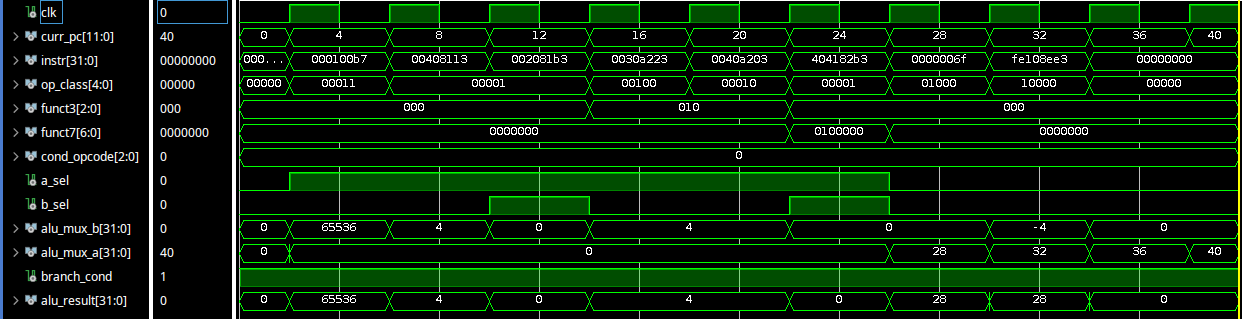
\includegraphics[scale=0.36]{IE_sim.png}
    \caption{Complete IE simulation}
    \label{fig:IE_sim}
\end{figure}

The testbench, following the step-by-step assembly of the whole datapath proposed in the ID section, can be built using a copy of the earlier code with the IE as an addition (Source Code \ref{code:IE_TB}).\\
Now when running a behavioral simulation the following events are expected to happen to be sure that the design is working properly: the first instruction is going to be encoded with \emph{op{\_}class} = "000110", while setting \emph{a{\_}sel} and pulling down \emph{b{\_}sel}, leaving \emph{alu{\_}result} = 65536, because LUI operation imply that the immediate operand is shifted by 16 bits to the left, thus multiplying it by $2^{15}$; The second one should sum the previous result with 4 and the folowing addition should return a 0, since the accessed register cannot yet be written; The following load, store and jump instructions should be performing additions, easy to notice from the ALU's output, which in case of SW and LW, should just return the immediate 4 summed to the registers that are still limited to store just zeroes, while jumps and branches sum the current PC's value to their orresponding immediate value (in Figure \ref{fig:IE_sim}).The subtraction is easily noticed by the fact that it represent the only one that changes \emph{funct7} and the last one should have the comparator set its only output:\\

